\chapter*{Appendix}
\addcontentsline{toc}{chapter}{Appendix}
\section*{Appendix Index}
\vspace{-8em}

% Adjust indentations before \listofanhang
\abstaendeanhangverzeichnis

\listofanhang
\clearpage
\spezialkopfzeile{Appendix} 

\lstset{
  language=TeX, % define keywords to highlight
  morekeywords={Appendix, anhangteil, anhan},
  breaklines=true,  % Enable line wrapping within the listing
  breakatwhitespace=true, % Breaks only at white space
  postbreak=\mbox{\textcolor{red}{$\hookrightarrow$}\space}, % Optional - for having a symbol at the point where text breaks
  basicstyle=\footnotesize\ttfamily, % for setting the font size/style for the code
  tabsize=2, % sets default tabsize
}


%% ================================== Discussion =======================================

\anhang{Discussion of Tool Evaluation and Weighing}

\anhangteil{Extensibility}

\anhangteil{Community, Support \& Docs}

This section assesses the level of external support provided for each project. To evaluate this support, we will focus on three distinct aspects and combine them into a single score. Firstly, we will examine the size of the community, as a substantial community often indicates project maturity and the availability of extensive support. As proxies for community size, we will consider two central metrics: the number of stars on GitHub and the quantity of questions on Stack Overflow.

\begin{table}[htb]
    \centering
    \caption{Comparison of Project Popularity}
    \label{tab:table1} 
    \begin{tabular}{|l|c|c|} 
      \textbf{Project} & \textbf{GitHub Stars} & \textbf{Stack Overflow Questions} \\ 
      Pachyderm  & 6,000   & 6          \\ 
      Argo       & 14,500  & 136        \\ 
      Clasp      & 0       & 0          \\ 
      Snaplogic  & 0       & 57         \\ 
      Airflow    & 32,200  & 10,218     \\ 
      Kubeflow   & 13,100  & 434        \\ 
      Knative    & 4,100   & 204        \\ 
      Luigi      & 16,900  & 346        \\ 
      CWL        & 1,400   & 6          \\ 
   \end{tabular}
\end{table}


\begin{figure}[htb]
    \centering
    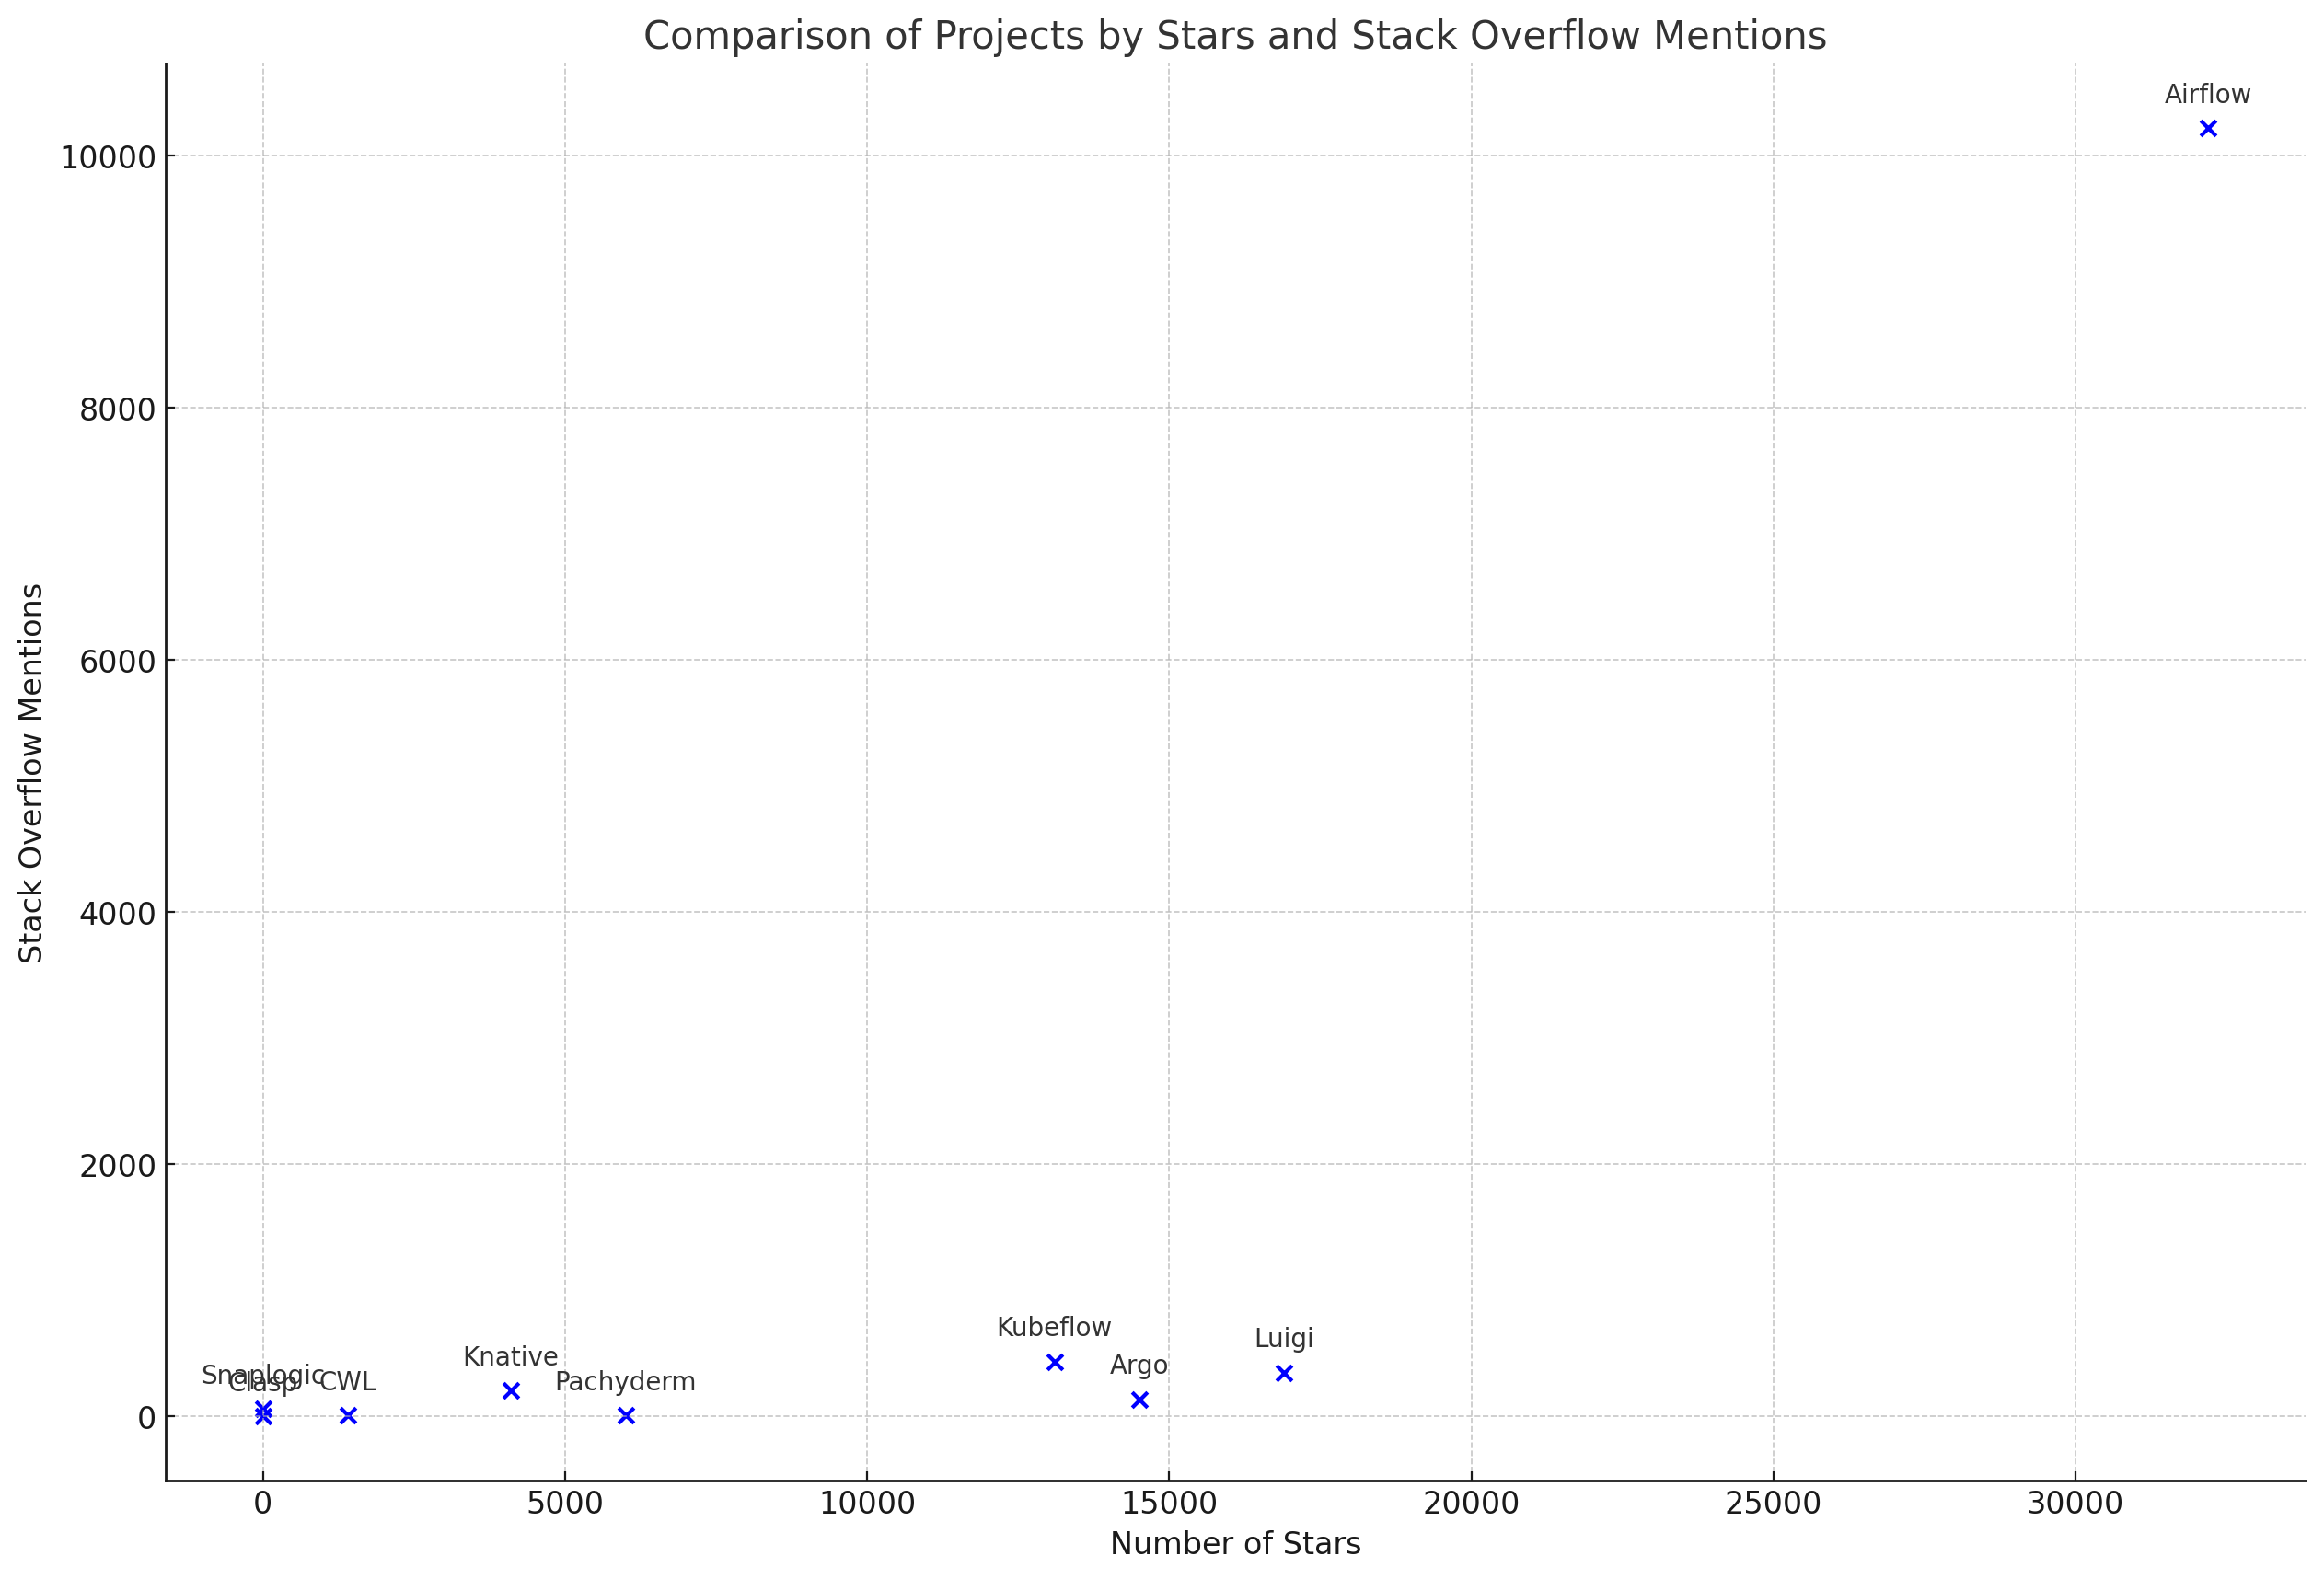
\includegraphics[width=12cm]{graphics/Stars_stackoverflow_comparison.png}
    \caption[Stars and Stackoverflow Questions Comparison]{Stars and Stack Overflow Questions Comparison}
    \label{abb:stars_stackoverflow_comparison}
\end{figure}

To gauge the level of support and community engagement surrounding these projects, we have devised a composite score that normalizes and combines the GitHub stars and Stack Overflow questions metrics. The calculation of this score involves the following methodology:

Each project is represented as a point \(P_i = (x_i, y_i)\) in a two-dimensional space, with \(x_i\) and \(y_i\) being the number of GitHub stars and Stack Overflow questions, respectively, for the \(i\)-th project. The composite score \(S_i\) for each project is computed by normalizing these values to a scale of 0-10 and then taking their average.

Additionally, we acknowledge that some commercial tools, as well as certain open-source projects, offer enterprise support, reducing the reliance on the community for assistance. Similarly, projects developed in-house often have access to the original development team for support. Therefore, we will apply a flat bonus of 5 points to the scores of projects offering enterprise support and a flat bonus of 2.5 points to projects developed in-house.

\[
S_i = \frac{1}{2} \left( \frac{x_i - \min(x)}{\max(x) - \min(x)} \times 10 + \frac{y_i - \min(y)}{\max(y) - \min(y)} \times 10 \right) + B_i
\]

Here, \(\min(x)\), \(\max(x)\), \(\min(y)\), and \(\max(y)\) represent the minimum and maximum values of GitHub stars and Stack Overflow questions across all projects, respectively. The final scores \(S_i\), along with the respective bonuses \(B_i\), provide a comprehensive metric for comparing project popularity, community engagement, and the availability of additional support options, all on the same scale.

\begin{table}[h!]
    \centering
    \begin{tabular}{|l|c|c|c|c|} 
    \hline
        \textbf{Project} & \textbf{Composite Score} & \textbf{Enterprise Bonus} & \textbf{Inhouse Bonus}  & \textbf{Final Score}\\
        \hline
        Airflow & 10.00 & 0 & 0 & 10.00 \\
        Pachyderm & 0.93 & 5 & 2.5 & 8.43 \\
        Snaplogic & 0.03 & 5 & 0 & 5.03 \\
        Luigi & 2.79 & 0 & 0 & 2.79 \\
        Clasp & 0.00 & 0 & 2.5 & 2.5 \\
        Argo & 2.32 & 0 & 0 & 2.32 \\
        Kubeflow & 2.25 & 0 & 0 & 2.25 \\
        Knative & 0.74 & 0 & 0 & 0.74 \\
        CWL & 0.22 & 0 & 0 & 0.22 \\
    \hline
    \end{tabular}
    \caption{Composite scores of Workflow managers, sorted by final score}
    \label{tab:results}
\end{table}


\anhangteil{License}

As discussed in section \ref{crit:license} the tools in consideration should not be to restrictive.
To evaluate the criteria we will employ a 4 bucket system: 
\begin{itemize}
    \item \textbf{Ideal Situation (Score: 10):} 
    This refers to cases where either the tool is in the public domain (and therefore not subject to copyright restrictions) or where our organization possesses a direct ownership or significant influence over the licensing terms.
    This situation provides the most flexibility, allowing for extensive modification, redistribution, and proprietary use without concern for licensing infringements.


    \item \textbf{Permissive License (Score: 7.5):}
    Tools under licenses like MIT, BSD, or Apache 2.0 fall into this category.
    These licenses are highly permissive and generally allow for broad freedom, including modification, distribution, and private use, with minimal restrictions, often limited to liability and warranty.

    \item \textbf{Restrictive or Reciprocal Licenses (Score: 2.5):}
    Licenses such as the GPL or AGPL are more restrictive, requiring any changes to be open-sourced or contributions to be made back to the community.
    These “copyleft” licenses can be problematic in proprietary settings where modifications or integrations need to remain confidential.

    \item \textbf{Unacceptable Licenses (Score: 0):}
    This includes licenses that impose burdensome conditions or high costs, proprietary software where the source code is unavailable, or situations where the licensing terms make it impractical to use within our projects.
    For instance, licenses that mandate the purchase of additional software, restrict certain types of use, or pose potential legal risks would fall into this category.
\end{itemize}

Now we will evaluate the licenses of the tools in question, and assign them a score based on the above criteria.

\begin{itemize}
    \item \textbf{Pachyderm} 
    The licensing model of Pachyderm follows a model which has similarities with the "Open Core model" \footcite{PahcydermPricing2022}.
    Which means that while the core functionalities are published as the "COMMUNITY EDITION" with a permissive source-available License (Apache License 2.0) \footcite{PachydermLICENSEMaster}.
    Functionality like \ac{SSO} or the ability to create more than 16 pipelines are part of a different distribution under a Commercial License.

    But in our case this is of no concern, as the startup behind the Pachyderm softwarem, including its \ac{IP} was aquired by \ac{HPE}.
    Giving us a free hand to modify without needing to worry.

    \item \textbf{Argo} 
    Argo's adoption of the Apache License 2.0 \footcite{ArgocdLICENSEMaster} aligns with common practices for open-source projects, affording users considerable freedom. This permissive license simplifies the use, modification, and redistribution of the software, an aspect that's particularly beneficial for collaborative development or integration into proprietary software. Given our requirements and operational context, this offers us the flexibility needed for adaptation and potential enhancements without stringent restrictions, streamlining any developmental efforts we undertake with Argo.
    \item \textbf{\ac{CLASP}} is not a published software and therefore not under any specific license.
    But similar considerations as the ones of Pachyderm apply here aswell, as it is an internal project the \ac{IP} also completely belongs to \ac{HPE}

    \item \textbf{Snaplogic} is an entirely commercial product which does not provide insight into nor the right to modify their Software \footcite{SnapLogicMasterSubscription}.
    But as they might agree this is not a total knockout criterion for this entire project, but in regards to the licensing it will be weighted with 0.
    \item \textbf{Airflow} is licensed under the Apache License 2.0. \footcite{LicenseAirflowDocumentation}
    \item \textbf{Kubeflow} is licensed under the Apache License 2.0. \footcite{KubeflowLICENSEMaster}
    \item \textbf{Knative} is licensed under the Apache License 2.0. \footcite{KnativeDocsLICENSE}
    \item \textbf{Luigi} is licensed under the Apache License 2.0. \footcite{LuigiLICENSEMaster}
    \item \textbf{CWL} is licensed under the Apache License 2.0. \footcite{CwlutilsLICENSEMain}
    
\end{itemize}

\anhangteil{Strategic alignment}

\anhangteil{Ease of Use}

\anhangteil{Maturity}

\anhangteil{Cost}



\begin{table}[htb]
    \centering
    \begin{tabular}{|l|l|l|l|l|} \hline
        \textbf{Criteria}                                          & \textbf{Pachyderm}    & \textbf{Argo}         & \textbf{\ac{CLASP}}   & \textbf{Snaplogic}     \\ \hline
        Ease of use                                                & TBD                   & TBD                   & TBD                   & TBD                    \\ \hline
        Extensibility                                              & TBD                   & TBD                   & TBD                   & TBD                    \\ \hline
        Community, Support \& Docs                                 & 10                   & 2.32                   & 2.5                   & 5.03                   \\ \hline
        Maturity                                                   & TBD                   & TBD                   & TBD                   & TBD                    \\ \hline
        Strategic alignment                                        & TBD                   & TBD                   & TBD                   & TBD                    \\ \hline
        License                                                    & 10                    & 7.5                     & 10                    & 0                      \\ \hline
        Cost                                                       & TBD                   & TBD                   & TBD                   & TBD                    \\ \hline

    \end{tabular}
    \caption{Evaluation of the suggested tools}
    \label{tab:evaluation_of_the_suggested_tools}
\end{table}



\begin{table}[htb]
    \centering
    \begin{tabular}{|l|l|l|l|l|l|} \hline
        \textbf{Criteria}                                          & \textbf{Airflow}      & \textbf{Kubeflow}     & \textbf{Knative}      & \textbf{Luigi}        & \textbf{CWL}          \\ \hline
        Ease of use                                                & TBD                   & TBD                   & TBD                   & TBD                   & TBD                   \\ \hline
        Extensibility                                              & TBD                   & TBD                   & TBD                   & TBD                   & TBD                   \\ \hline
        Community, Support \& Docs                                 & 10                    & 2.25                  & 0.74                  & 2.29                  & 0.22                  \\ \hline
        Maturity                                                   & TBD                   & TBD                   & TBD                   & TBD                   & TBD                   \\ \hline
        Strategic alignment                                        & TBD                   & TBD                   & TBD                   & TBD                   & TBD                   \\ \hline
        License                                                    & 7.5                     & 7.5                     & 7.5                     & 7.5                     & 7.5                     \\ \hline
        Cost                                                       & TBD                   & TBD                   & TBD                   & TBD                   & TBD                   \\ \hline

    \end{tabular}
    \caption{Evaluation of the additional tools}
    \label{tab:evaluation_of_the_additional_tools}
\end{table}

%% ============================== Diagrams =====================================

\newpage
\anhang{Diagrams}

\anhangteil{Pipeline Communication Swim Lane Diagram}
\label{appendix:pipeline_communication_sld}

\begin{figure}[htb]
  \centering
  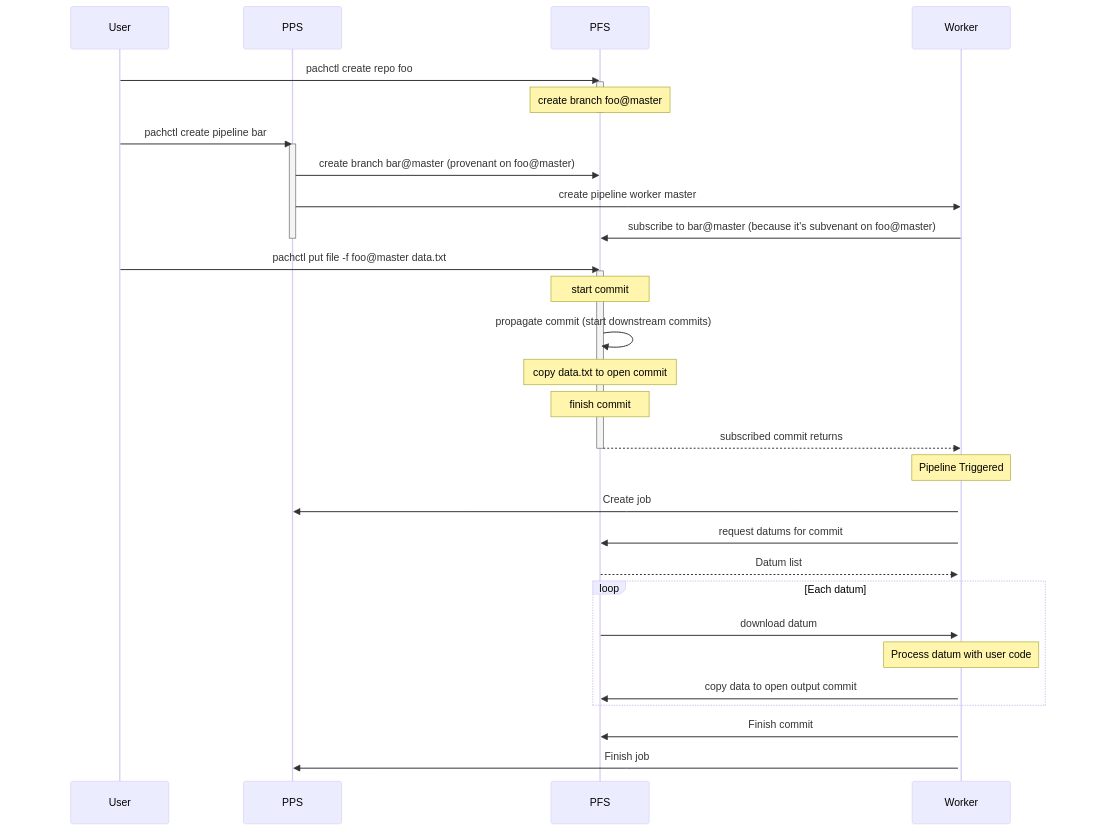
\includegraphics[width=17cm]{graphics/pipeline_communication_sld.png}
  \caption[Swimlane Diagram of the communication between the user and Pachyderm]{Swimlane Diagram of the communication between the user and Pachyderm}
  \label{abb:pipeline_communication_sld}
\end{figure}
\footnotetext{Taken from: \cite{IntroPipelines2023}}

\newpage

%% ================================ Code =======================================


\anhang{Minikube installation instructions}
\label{appendix:minikube_installation_instructions}
\lstinputlisting{../quellen/minikube_installation_instructions.md}

\newpage
\anhang{Kubernetes setup scripts}

\anhangteil{Ansible setup script}
\label{appendix:ansible_setup_script}
\lstinputlisting{../../Project/Kubernetes_Setup/kluster/setup_scripts/join_cluster.yaml}

\newpage
\anhangteil{Flannel configuration}
\label{appendix:flannel_config}
\lstinputlisting{../../Project/Kubernetes_Setup/kube-flannel.yml}

% \anhangteil{Bash setup script}
% \label{appendix:bash_setup_script}
% \lstinputlisting{../../Project/Kubernetes_Setup/kluster/setup_scripts/setup.sh}

\newpage
\anhangteil{Bash verification script}
\label{appendix:bash_verification_script}
\lstinputlisting{../../Project/Kubernetes_Setup/kluster/setup_scripts/double_check.sh}

\newpage
\anhangteil{Arkouda Setup}
\label{appendix:arkouda_setup}
\lstinputlisting{../../Project/Kymera/README.md}